% Chapter Template

\chapter{Design and Implementation of Inference Engine}\doublespacing % Main chapter title

\label{Chapter3} % Change X to a consecutive number; for referencing this chapter elsewhere, use \ref{ChapterX}

\lhead{Chapter III. \emph{Design and Implementation of Inference Engine}} % Change X to a consecutive number; this is for the header on each page - perhaps a shortened title

%----------------------------------------------------------------------------------------
%	SECTION 1
%----------------------------------------------------------------------------------------
\section{Introduction}
A typical inference engine should perform operations like convolution, max pooling, non linear activation and padding. Apart from this, there are other modules which are required for accessing data from memory. They are in charge of retrieving the inputs and kernels from memory. They are assisted by the readModules, which are linked via a deadlock prevention system. The retrieved data is sent through pipes to the compute convolution module, where the main computations take place. The partial sums are then gathered in the accumulator. Subsequently, the outputs are produced by quantizing and applying activation functions before being written back to memory.\\
% \newpage
The engine's primary requirement is to perform all the aforementioned operations with high throughput. To achieve that, the critical modules of the accelerator should run at full rate.

\begin{figure}[h]
    \centering
    % \includegraphics[width=\linewidth]{Chapters/Chapter_3/images/Overview.png}
    \includegraphics[width=\linewidth]{../figures/Overview.png}
    \caption{Block diagram for the engine implementation}
    % \label{fig:your_label}
\end{figure}
% Hello
\section{Fetch Module}
This module ensures a continuous data stream to the compute module. A series of submodules were designed to optimize input delivery rates, enabling the compute module to operate at maximum throughput without data stalls during each computation stage.
\subsection{Fetch Input Initial}
% Before starting the compute module, initially ( $k_r$ x $k_c$ x chn )($k_r$ and $k_c$ are kernel row \& columns and chn is the number of input channels) elements are fetched from the memory and stored in the internal pipes in\_data\_<i>, where i is the column number of the image. These pipes are read by Input Data Loader to provide steady stream of data to the multiplier used in the compute dot product module. Since we need to reuse the input data to reduce multiple memory access, we also re write the required data into the in\_data\_<i> pipes.
Prior to initiating the Compute Module, an initial batch of ( $k_r$ x $k_c$ x chn )($k_r$ and $k_c$ are kernel row \& columns and chn is the number of input channels) elements is pre-fetched from memory and stored in the internal pipes, denoted as in\_data\_<i>, where i represents the column index of the image. These pipes are subsequently read by the Input Data Loader module to provide a sustained and high-throughput supply of data to the multiplier unit within the Compute Dot Product Module. To minimize memory access and maximize data reuse, a data rewriting mechanism is employed, wherein the required data elements are re-written into the in\_data\_<i> pipes, ensuring optimal data locality and reducing memory access latency.
\subsection{Fetch Kernel}
% Similar to fetch input initial, fetch kernel also stores the ( $k_r$ x $k_c$ x chn ) elements in ker\_data pipe before starting the compute module. Once both the sub modules are executed, the compute module is initialized along with the fetch input partial sub module, to stream the remaining input data to the engine.
Analogous to the fetch input initial phase, the fetch kernel module preloads the ( $k_r$ x $k_c$ x chn ) elements in ker\_data pipe, prior to initializing the Compute Module. Upon completion of both the fetch input initial and fetch kernel sub-modules, the Compute Module is activated, in conjunction with the fetch input partial sub-module, to stream the remaining input data to the processing engine, ensuring a continuous and high-throughput data flow. 
\subsection{Fetch Input Partial}
% Since the compute module already have ( $k_r$ x $k_c$ x chn ) elements for processing the output, we need to reuse ( ($k_r$) x ($k_c$ - 1) x chn ) elements as the kernel strides forward. So before the computation of the next output starts,  we just need to fetch ( $k_r$ x chn ) elements and store it on the pipes. By doing this, the compute module will run at full rate and need not wait for last column at each computation stage.

Due to the Compute Module already possessing the requisite ( $k_r$ x $k_c$ x chn ) elements for processing the current output, a data reuse strategy is employed to maximize computational efficiency. Specifically, ($k_r$) x ($k_c$ - 1) x chn ) elements are reused as the kernel strides forward, thereby reducing the data fetch requirement. Consequently, prior to initiating the computation of the subsequent output, only ( $k_r$ x chn )  elements need to be fetched and stored in the pipes, ensuring that the Compute Module operates at its peak throughput without experiencing any data starvation or wait states during each computation stage.


\subsection{De-Quantization}
Since the data retrieved from memory is represented in an 8-bit unsigned integer format (uint8), a format conversion is necessitated to transform the data into single-precision floating-point numbers (FP32) to facilitate the computation stage. This format conversion is achieved through the application of the De-Quantization formula, as specified by the PyTorch Framework, which involves a scaling operation that multiplies the quantized integer values by a scalar factor, denoted as the scale, and a subsequent addition of a zero-point offset, thereby effectively converting the quantized data to its original floating-point representation.
\begin{equation*}
\text{Inp}_{\text{de-quantized}} = \text{scale\_factor} \times (\text{Inp}_{\text{quantized}} - \text{zero\_point})
\end{equation*}
where \( \text{zero\_point} \) is the zero-point offset and \( \text{scale\_factor} \) is the scaling factor.


\section{Compute Module}
% Since this module forms the core of the engine, the throughput of the engine depends on the rate at which this module will run. The submodules present in this ensure that the compute module will run at full rate.
Given that the Compute Module serves as the engine's core processing unit, its performance has a direct impact on the engine's overall throughput. The submodules embedded within this module are carefully designed to ensure that the Compute Module maintains an optimal execution rate, thereby enabling the engine to operate at its maximum processing capacity and achieve peak performance.
\subsection{Compute Dot Product}
% The dot product submodule contains a single 32 bit floating point multiplier. This submodule reads the data from input loader and kernel loader, and then pushes the dot product of both into accumulator. Since number of dot products will be fixed, using the formula ($k_r$ * $k_c$ * chn) * ($o_r$ * $o_c$), ( $o_r$ and $o_c$ are number of output rows and columns), this submodule expects these number of elements from input and kernel loader to perform dot product.
The Dot Product Submodule, a crucial component of the Compute Module, incorporates a single 32-bit floating-point multiplier, which facilitates the computation of the dot product between the input data and kernel coefficients. This submodule retrieves the requisite data from the Input Loader and Kernel Loader modules, and subsequently performs the dot product operation, yielding a result that is will be accumulated. The number of dot product operations is predetermined, and is calculated using the formula ($k_r$ * $k_c$ * chn) * ($o_r$ * $o_c$), ( $o_r$ and $o_c$ are number of output rows and columns).Accordingly, the Dot Product Submodule expects to receive a specific number of elements from the Input Loader and Kernel Loader modules, which is necessitated for the efficient computation of the dot product.
\subsection{Compute Accumulator}
% The accumulator also expects ($k_r$ * $k_c$ * chn) * ($o_r$ * $o_c$) elements from the dot product submodule. In addition to this, the accumulator module should also be aware of when to send the accumulated value to the output module. Since a output pixel is generated from summation of ($k_r$ * $k_c$ * chn) dot products between input and kernel, hence the accumulator sends the accumulated value after accumulating  ($k_r$ * $k_c$ * chn) elements and then restarts the accumulator process for the next output pixel.
The Accumulator Module, a critical component of the Compute Engine, expects to receive a predetermined number of elements from the Dot Product Submodule, specifically ($k_r$ * $k_c$ * chn) * ($o_r$ * $o_c$) elements. Additionally, the Accumulator Module is designed to intelligently manage the accumulation process, recognizing when to forward the accumulated value to the Output Module, which occurs after the summation of ($k_r$ * $k_c$ * chn) dot products between input and kernel coefficients. This triggers the accumulator reset, initiating the accumulation process anew for the subsequent output pixel, thereby ensuring efficient and accurate processing of output data.
\subsection{Input and Kernel Loader}
% These submodules read the data stored in the internal pipes by the Fetch module and supply it to the dot product submodule in the correct sequence. They are also responsible for data reutilization; once the data is accessed from the in\_data and ker\_data pipes, it is rewritten back to these pipes in the appropriate order to minimize frequent memory accesses.
The Input Data Loader and Kernel Data Loader submodules, integral components of the Compute Engine, are responsible for reading data from the internal pipelines, specifically the in\_data and ker\_data pipes, which are populated by the Fetch Module. These submodules ensure that the data is supplied to the Dot Product Submodule in a precise and sequential manner, thereby facilitating efficient computation. Moreover, they implement a data reutilization strategy, wherein the accessed data is rewritten back to the internal pipelines in a specific order, minimizing frequent memory access and reducing the associated latency, thus optimizing the overall performance of the Compute Engine.

% \subsection{Kernel Loader}

% \section{Quantization Operations}


% \section{Non Critical Components}
% \subsection{Input Module}
% \subsection{Kernel Module}
% This module handles the retrieval of kernel data from memory and transfers it to the compute module. Since the kernel size (k) in our application is atmost 5, so we fetch k x k x chn (chn is the number of input channels) elements from the memory and store it in on-chip buffer. This data is re used for processing the entire input before discarding them from on-chip buffers.
\section{Output Module}
The output modules receive data from the accumulator, perform necessary operations on them, and subsequently store the results back into memory.
\subsection{Non Linear Activation}
Upon receiving of the data, the module applies the Rectified Linear Unit (ReLU) activation function, contingent upon the activation of the corresponding non-linearity flag. The operation is executed on the accumulated outputs prior to  quantization and then written back to the memory.

\subsection{Pooling}
% The output modules additionally execute maxpooling following convolution. Since we are performing 2 x 2 max pooling, we store two rows of output data and then perform max pooling operation on the output data before writing them back to the memory.
The Output Modules additionally perform max pooling operations subsequent to convolution, implementing a 2 x 2 max pooling kernel. In order to facilitate this operation, two rows of output data are buffered and temporarily stored, followed by the execution of the max pooling algorithm, which selects the maximum values from the pooled regions. The resultant output data is then written back to memory, thereby reducing spatial dimensions and retaining essential features.

\subsection{Quantization}
% After completion of the non linear activation, the 32 bit float is then converted to the 8 bit uint format using the quantization formula provided by PyTorch Framework. The quantization formula involves scaling the floating-point values by a scale factor and adding a zero-point offset, followed by rounding to the nearest integer.
Following the completion of the non-linear activation, the 32-bit floating-point numbers are subsequently quantized to 8-bit unsigned integers (uint8) using the quantization formula prescribed by the PyTorch Framework, which entails a scaling operation that multiplies the floating-point values by a scalar factor, followed by the addition of a zero-point offset, and culminates in a rounding operation to the nearest integer, thereby effecting a precise conversion from floating-point to integer representation.
\begin{equation*}
\text{Out}_{\text{quantized}} = \text{round}\left( \frac{\text{Out}_{\text{float}}}{\text{scale\_factor}} + \text{zero\_point} \right)
\end{equation*}
where \( \text{zero\_point} \) is the zero-point offset and \( \text{scale\_factor} \) is the scaling factor.

% \subsection{Read and Write Modules}
% These modules serve as interfaces between functional pipes and the memoryModule. They facilitate read and write operations to memory by providing addresses and/or data along with appropriate bitmasks. Upon completion of a memory load operation, they return the read data to the calling module.\\
% While there are no cyclic dependencies among the core modules, they share a single resource—memory—accessible through the memoryModule. This shared resource poses a potential risk of deadlock, where one module may block another due to pipe dependencies. For instance, if the input module is blocked by pipe constraints, it can hinder the readModule's ability to retrieve data from memory, consequently causing memory blockage that prevents writeback operations from completing. This domino effect can ultimately lead to deadlock, where all modules become blocked.\\
% To mitigate deadlocks arising from shared resource contention, the read modules employ a mechanism illustrated in Figure 3.5. This mechanism ensures that the number of active iterations in readModule1 is limited by the pipe depth of 7. Consequently, the pipe can accommodate a maximum of 7 entries in the PIPE at any given time, preventing blocking scenarios. Thus, each memory access initiated by readModule1 is guaranteed to return, effectively averting resource contention and potential deadlocks.\\
% It's important to note that deadlock prevention mechanisms are not necessary for writeModules. This is because output from the writeModule does not pass through a pipe and therefore never encounters blocking situations.

% \subsection{Memory Module}
% The module serves as an intermediary between the engine and external memory. It handles read/write requests from other modules via their respective interfaces, transmitting a 110-bit request to the ahir core bus (ACB). The ACB forwards this request to the memory controller for access, which returns a 65-bit response containing a 1-bit error flag and 64-bit data. This response is then relayed back to the originating module. The memory module abstracts the system design from the memory interface, utilizing the ACB interface. This allows the engine to manage read/write operations—specifying flags, data, address, and bytemask—without needing to manage the specifics of the underlying memory technology (such as BRAM/DRAM).
\section{Interface to Access The Accelerator}
Two continuously operating daemons manage the engine. The first is the accelerator\_control\_daemon, responsible for initializing registers, launching the worker daemon, and receiving configuration details from the processor or calling module via the AFB interface. Using this information, it configures the registers accordingly.

The second daemon is the accelerator\_worker\_daemon, which monitors the control register R0. It continuously checks until bits 0 and 2 are set by the calling module. Upon meeting this condition, it reads the remaining registers and triggers the convolution engine through a command call.

The convolution engine function call is represented as:\\
\$call convengine (\\
\hspace*{1cm} in\_start\_addr \quad out\_start\_addr \quad  ker\_start\_addr \quad out\_grp\_no \quad in\_rows\\
\hspace*{1cm} in\_cols \quad in\_channels \quad  out\_channels \quad groups \quad ker\_size \quad pool\_cols\quad inp\_scale \\
\hspace*{1cm} inp\_zero\_point \quad ker\_scale \quad  ker\_zero\_point \quad conv\_scale \quad conv\_zero\_point\\
\hspace*{1cm} padReq \quad poolReq \quad  isLinear \quad isActivation \quad isFlatten \quad flattenOffset \quad out\_chn\_ind\\
\hspace*{1cm} ) \quad ()

where:
\begin{itemize}
    \item \textbf{in\_start\_addr}: Starting address of the input data.
    \item \textbf{out\_start\_addr}: Starting address where the output data will be stored.
    \item \textbf{ker\_start\_addr}: Starting address of the kernel data.
    \item \textbf{out\_grp\_no}: Output group number.
    \item \textbf{in\_rows}: Number of rows in the input data.
    \item \textbf{in\_cols}: Number of columns in the input data.
    \item \textbf{in\_channels}: Number of input channels.
    \item \textbf{out\_channels}: Number of output channels.
    \item \textbf{groups}: Number of groups in the convolution.
    \item \textbf{ker\_size}: Size of the kernel.
    \item \textbf{pool\_cols}: Pooling columns.
    \item \textbf{inp\_scale}: Input scaling factor.
    \item \textbf{inp\_zero\_point}: Input zero point.
    \item \textbf{ker\_scale}: Kernel scaling factor.
    \item \textbf{ker\_zero\_point}: Kernel zero point.
    \item \textbf{conv\_scale}: Convolution scaling factor.
    \item \textbf{conv\_zero\_point}: Convolution zero point.
    \item \textbf{padReq}: Padding requirement.
    \item \textbf{poolReq}: Pooling requirement.
    \item \textbf{isLinear}: Flag indicating if the operation is linear.
    \item \textbf{isActivation}: Flag indicating if activation is applied.
    \item \textbf{isFlatten}: Flag indicating if flattening is performed.
    \item \textbf{flattenOffset}: Offset used for flattening.
    \item \textbf{out\_chn\_ind}: Output channel index.
\end{itemize}

\subsection{Register File Format}
The accelerator engine utilizes 16 registers of 32-bit each for communication with external interfaces, facilitating the exchange of specific information as follows:
\begin{itemize}
    \item Register 0: Functions as the controller for the accelerator and monitors status flags.
    \item Register 1: Stores the base address for the input tensor
    \item Register 2: Stores the base address for the output tensor
    \item Register 3: Stores the base address for the kernel tensor
    \item Register 4: The index of the current output group
    \item Register 5: Stores the value of the number of input rows (31 downto 16) and
number of input columns (15 downto 0)
    \item Register 6: Stores the value of the number of input channels (31 downto 16) and
number of input groups (15 downto 0)
    \item Register 7: Stores the kernel size
    \item Register 8: Stores the number of columns present in the pooling layer
    \item Register 9: Stores the base address for scale and zero point values required for the quantization functions
    \item Register 10: Stores the control for padding (bit 4), pooling (bit 3), linear convolution (bit 2), activation (bit 1) and flatten (bit 0)
    \item Register 11: Stores the value of the number of output channels (31 downto 16) and
current index of the output (15 downto 0)
    \item Register 12: Stores the offset address required during flattening of the output tensor
\end{itemize}
Registers 13-15 are currently unused but can be repurposed for additional parameters or for debugging purposes.\\
Register 0 has the following bits used:
\begin{itemize}
    \item Bit 0: "accl enable" controls the activation of the engine and can be toggled externally.
    \item Bit 1: "interrupt enable" sets or clears the interrupt flag, which can be controlled by invoking the module.
    \item Bit 2: The "start cmd" is triggered by invoking the module, directing the accelerator to commence execution.
    \item Bit 3: "cmd complete" is set by the accelerator to signify the completion of execution, and it is reset by the processor when preparing to signal the next command.
    \item Bit 4: "accl done" is activated by the accelerator to indicate the completion of execution and prompt the generation of an interrupt.
\end{itemize}
\newpage
\section{Resource Utilitzation}

\begin{table}[h]
    \centering
    \begin{tabularx}{1.1\textwidth}{|X|X|X|r|r|r|X|}
        \hline
        \textbf{Reference} & \textbf{Quantization Method} & \textbf{Clock}  & \textbf{LUTs} & \textbf{DSP} & \textbf{FF} & \textbf{Accuracy} \\
        \hline
        [2]Mohd, Bassam et.al & Quantization Aware Training (QAT) &200 MHz  & 50k  & -  & - & 96.67\% \\\hline
        
        [3] Blott, Michaela et.al & FINN &250 MHz  & 67k  & 0  & - & 98.8\% \\\hline
        [4] Ji, Mengfei et.al & FPQNet &250 MHz  & 53k  & 2614  & 94k & 98.8\% \\\hline
        This Work & FINN &125 MHz  & 67k  & 183  & 74k & 98\% \\\hline

   
    \end{tabularx}
    \caption{Resource utilization and comparison with other work}
    \label{tab:PTQ_comparison}
\end{table}
% Nam dui ligula, fringilla a, euismod sodales, sollicitudin vel, wisi. Morbi auctor lorem non justo. Nam lacus libero, pretium at, lobortis vitae, ultricies et, tellus. Donec aliquet, tortor sed accumsan bibendum.


% \section{Methodology}
% Lacus libero, pretium at, lobortis vitae, ultricies et, tellus. Donec aliquet, tortor sed accumsan bibendum Figure \ref{fig:figure3_1}.

% \lipsum[2]
 
% % adjustbox is used to limit the figure inside the page
% -- means normal arrow
%  -| horizontal then vertical arrow
%  |- vertical then horizontal arrow


\begin{figure}[!ht]

    \begin{center}
        \begin{adjustbox}{max height=0.8\textheight, center, width=0.6\textwidth}
            \begin{tikzpicture}[node distance=2.5cm]
                \node (t1) [startstop] {\textbf{{\Large Step 1}}};
                \node (t2) [process, below of = t1] {\textbf{{\Large Step 2}}};
                \node (t3) [process, below of = t2] {\textbf{{\Large Step 3}}};
                \node (t4) [process, below of = t3] {\textbf{{\Large Step 4}}};
                \node (t5) [process, below of = t4] {\textbf{{\Large Step 5}}};
% ---------------------------------------------
% vertical (primary) Division
% ---------------------------------------------
                % Flow

                \node (t6) [process, below of = t5] {\textbf{{\Large Step 6}}};

                \node (t7) [process, below of = t6] {\textbf{{\Large Step 7}}};

                \node (t8) [process, below of = t7] {\textbf{{\Large Step 8}}};

                \node (t9) [process, below of = t8] {\textbf{{\Large Step 9}}};

                \node (t10) [process, below of = t9] {\textbf{{\Large Step 10}}};

                \node (t11) [process, below of = t10] {\textbf{{\Large Step 11}}};

                 \node (t12) [process, below of = t11] {\textbf{{\Large Step 12}}};


% ---------------------------------------------
% All arrows (for vertical column
% ---------------------------------------------

                %  All arrows (for vertical column
                \draw [arrow] (t1) -- (t2);
                \draw [arrow] (t2) -- (t3);
                \draw [arrow] (t3) -- (t4);
                \draw [arrow] (t4) -- (t5);
                \draw [arrow] (t5) -- (t6);
                \draw [arrow] (t6) -- (t7);
                \draw [arrow] (t7) -- (t8);
                \draw [arrow] (t8) -- (t9);
                \draw [arrow] (t9) -- (t10);
                \draw [arrow] (t10) -- (t11);
                \draw [arrow] (t11) -- (t12);
% ---------------------------------------------
% Left Division
% --------------------------------------------- 
                \node (l1) [process, left of = t5, xshift=-10cm, yshift=-2.6cm] {\textbf{{\Large Left 1}}};

                \node (l2) [process, below of = l1, yshift=-0.3cm] {\textbf{{\Large Left 2}}};
                

% ---------------------------------------------
% All arrows (for the left column)
% ---------------------------------------------

                %  All arrows (for vertical column
                \draw [arrow] (t5) -| (l1);
                \draw [arrow] (l1) -- (l2);
                \draw [arrow] (l2) |- (t8);

% ---------------------------------------------
% Right Division
% ---------------------------------------------   
                \node (r1) [process, right of = t8, xshift=10cm, yshift=-4cm] {\textbf{{\Large Right 1}}};

% ---------------------------------------------
% All arrows (for right column)
% ---------------------------------------------

                %  All arrows (for vertical column
                \draw [arrow] (t8) -| (r1);
                \draw [arrow] (r1) |- (t11);
                
            \end{tikzpicture}
        \end{adjustbox}
    \end{center}
    \caption{Study methodology.}
    \label{fig:figure3_1}
\end{figure}


% \section{Models and Algorithms}
% \lipsum[1]

% Here is equation \ref{Eq3_1}.

% % Equation
% \begin{equation}
% e = \lim_{n\to\infty} \left(1+\frac{1}{n}\right)^n
% \label{Eq3_1}
% \end{equation} 

% \begin{align}
% 	x^2 -25 &= 0 \nonumber \\
% 	x^2 &= 25 \nonumber \\
% 	\therefore \Aboxed{x &= 5}
%  \label{Eq3_2}
% \end{align}



% \begin{multline}
% 	f(x) = 4xy^2 + 3x^3 - 2xy + 25x^3y^3 + 3xy - 4x^6y^6 + 3xy^2 - 2y^3\\ + a^3b^3c^4 + 3x^3 - 2xy + 25x^3y^3 + 3xy\\ - 4x^6y^6 + 3xy^2 - 2y^3 + a^3b^3c^4
% \label{Eq3_3}
% \end{multline}

% \section{Summary}
% \lipsum[2]
